\documentclass[a4paper]{article}

\usepackage[utf8]{inputenc} %- Løser problem med å skrive andre enn engelske bokstaver f.eks æ,ø,å.
\usepackage[T1]{fontenc} %- Støtter koding av forskjellige fonter.
\usepackage{textcomp} % Støtter bruk av forskjellige fonter som dollartegn, copyright, en kvart, en halv mm, se http://gcp.fcaglp.unlp.edu.ar/_media/integrantes:psantamaria:latex:textcomp.pdf
\usepackage{csquotes}
\usepackage{url} % Gjør internett- og e-mail adresser klikkbare i tex-dokumentet.
\usepackage{hyperref} % Gjør referansene i tex-dokumentet klikkbare, slik at du kommer til referansen i referanselista.
\usepackage[english]{babel} % Ordbok. Hvis man setter norsk i options til usepackage babel kan man bruke norske ord.
\usepackage{amsmath} 				% Ekstra matematikkfunksjoner.
\usepackage{amssymb}
\usepackage{amsfonts}
\usepackage{amsthm}
\usepackage{mathrsfs}
\usepackage{mathtools}
\usepackage{geometry}
\usepackage{tikz-cd}
\usepackage{graphicx}
\usepackage{changepage}
\usepackage{subcaption}
\usepackage{placeins}
\usepackage{bm}
\usepackage{physics}
\usepackage{siunitx}					% Må inkluderes for blant annet å få tilgang til kommandoen \SI (korrekte måltall med enheter)
	\sisetup{exponent-product = \cdot}      	% Prikk som multiplikasjonstegn (i steden for kryss).
 	\sisetup{output-decimal-marker  =  {,}} 	% Komma som desimalskilletegn (i steden for punktum).
 	\sisetup{separate-uncertainty = true}   	% Pluss-minus-form på usikkerhet (i steden for parentes). 
\usepackage{booktabs} % For å få tilgang til finere linjer (til bruk i tabeller og slikt).
\usepackage[font=small,labelfont=bf]{caption}		% For justering av figurtekst og tabelltekst.
\usepackage[backend=biber]{biblatex}
\addbibresource{./ref.bib}

% math stuff
\newcommand{\restr}[2]{\ensuremath{\left.#1\right|_{#2}}}

% my personal commands
\newcommand{\R}{\mathbb{R}}

%\clearpage % Bruk denne kommandoen dersom du vil ha ny side etter det er satt plass til figuren.
% Disse kommandoene kan gjøre det enklere for LaTeX å plassere figurer og tabeller der du ønsker.
\setcounter{totalnumber}{5}
\renewcommand{\textfraction}{0.05}
\renewcommand{\topfraction}{0.95}
\renewcommand{\bottomfraction}{0.95}
\renewcommand{\floatpagefraction}{0.35}

% math stuff
\newtheorem{theorem}{Theorem}
\newtheorem{claim}[theorem]{Claim}
\newtheorem{proposition}[theorem]{Proposition}
\newtheorem{lemma}[theorem]{Lemma}
\newtheorem{corollary}[theorem]{Corollary}
\newtheorem{conjecture}[theorem]{Conjecture}
\newtheorem*{observation}{Observation}
\newtheorem*{example}{Example}
\newtheorem*{remark}{Remark}

\graphicspath{{../}}

\title{Project for Deep Learning in Scientific Computing}

\author{Alexander Johan Arntzen }

\date{\today}

%%%%%%%%%%%%%%%%%%%%%%%%%%%%%%%%%%%%%%%%%%%%%%%%%%%%%%%%%%%%%%%%%%%%%%%%%
\begin{document}

\maketitle

\section*{Task 1}
In this task a noisy dataset was provided. Attempts to denoise the data did not produce a better cross validation error, so no denoising was used. All the data was then normalized by min-max normalization.

A feed forward fully connected neural network was chosen to approximate the map. Training was then performed to select the optimal hyperparameters using cross validation error as a selection criterion. The final model was trained 10 times, and the lowest validation error was chosen. The resulting approximation is plotted in Figure \ref{fig:task1}

\begin{figure}[b]
	\begin{subfigure}[b]{0.5\textwidth}
	  \centering
	  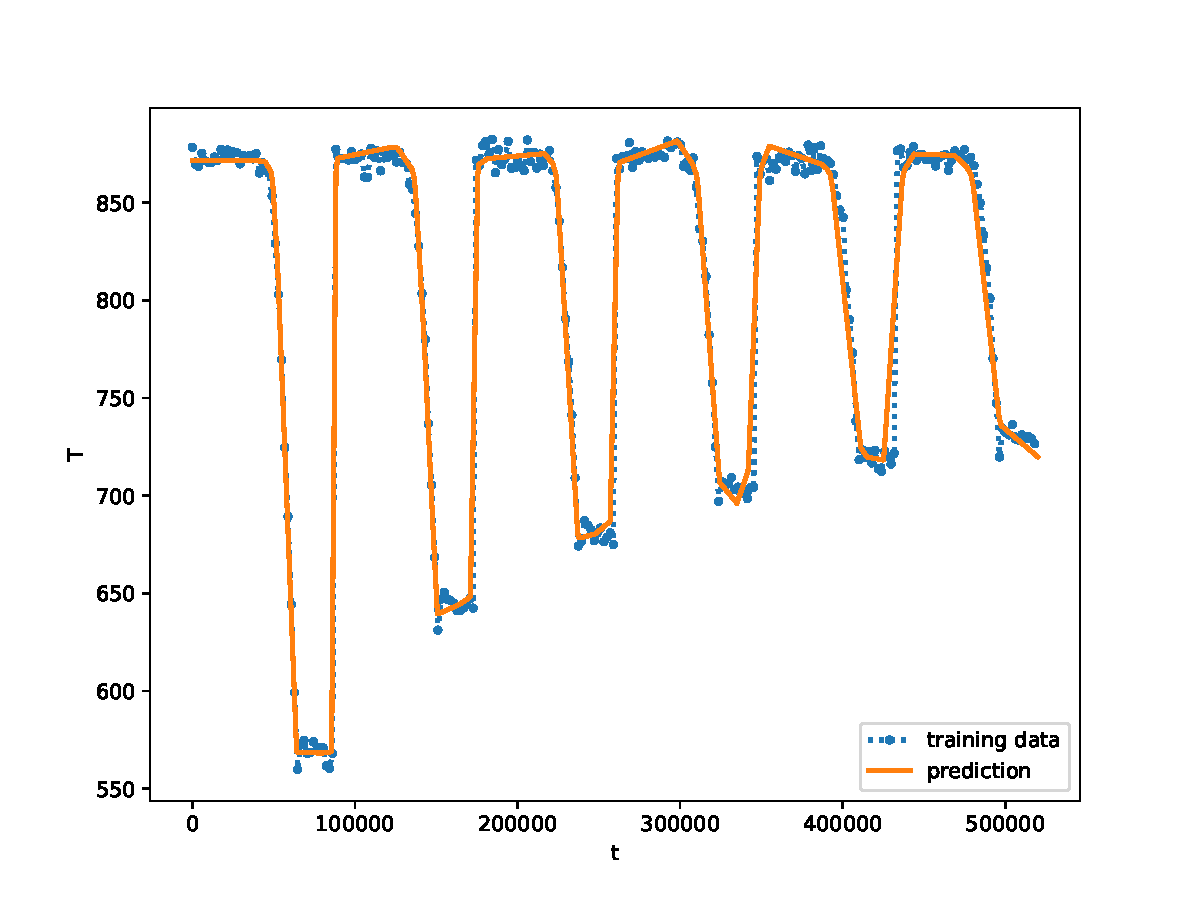
\includegraphics[width=\linewidth]{figures/task1/final_tf0.pdf}
	  \caption{$T_f^0$}
	  \label{fig:task1a}
	\end{subfigure}
	\begin{subfigure}[b]{0.5\textwidth}
	  \centering
	  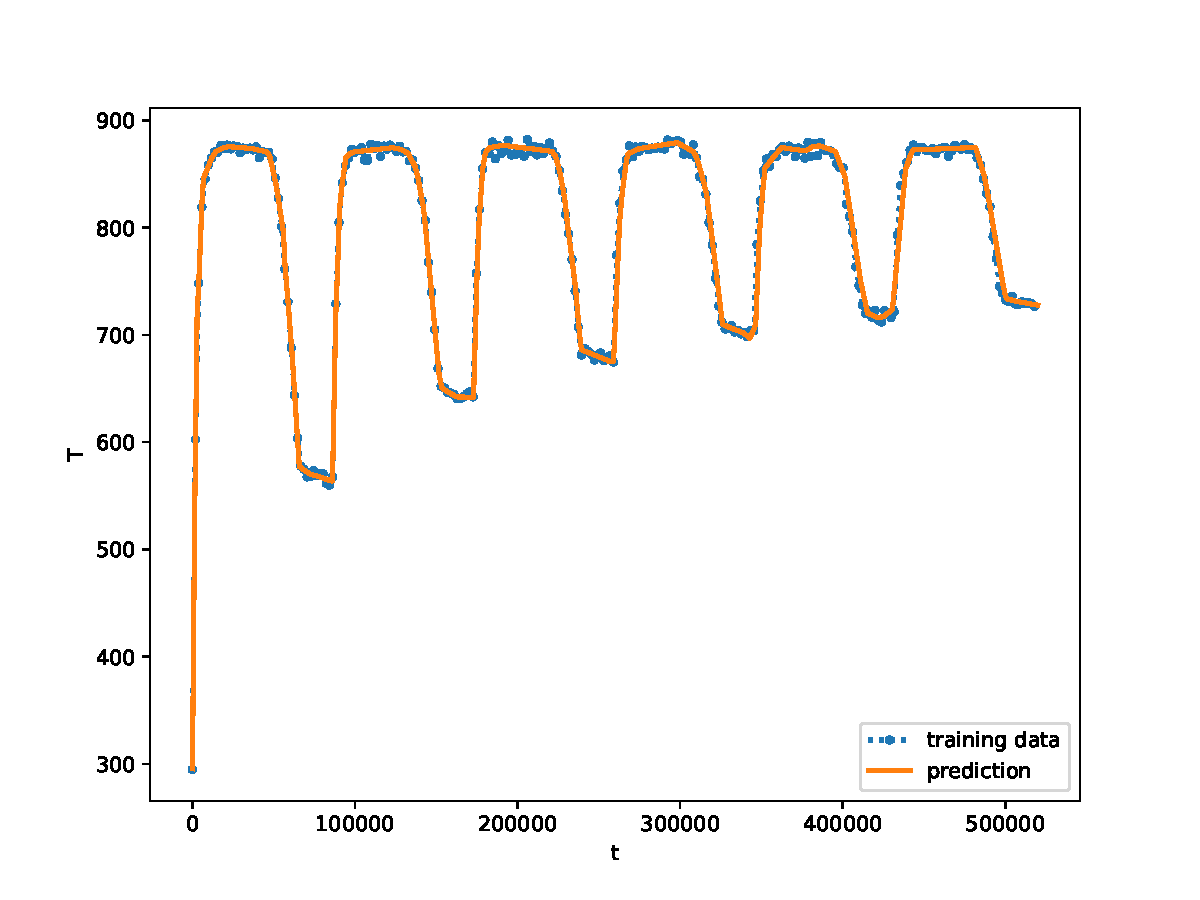
\includegraphics[width=\linewidth]{figures/task1/final_ts0.pdf}
	  \caption{$T_s^0$}
	  \label{fig:task1b}
	\end{subfigure}
	\caption{Training points and approximation made by the model}
	\label{fig:task1}
  \end{figure}

\section*{Task 2}
In this task both the Sobol points and the transformed points were given. By using linear regression, the parameters of the transformation was found. It was then observed that the points used in the finest mesh solutions also existed in the coarser solutions. Thus, it was possible to use the more accurate $CF$ values where they where available. The $CF$ values where then standardized, since they approximated a normal distribution. 
Training a feed forward fully connected neural network on the aggregated data gave better results than a multilevel\cite{lye2020multilevel} approach. Ensemble training was then performed to select the optimal hyperparameters using cross validation error as a selection criterion. The final model was trained 10 times, and the lowest validation error was chosen. A plot of the predicted $CF$ values can be found in Figure \ref{fig:task2}  
\begin{figure}[ht]
    \centering
    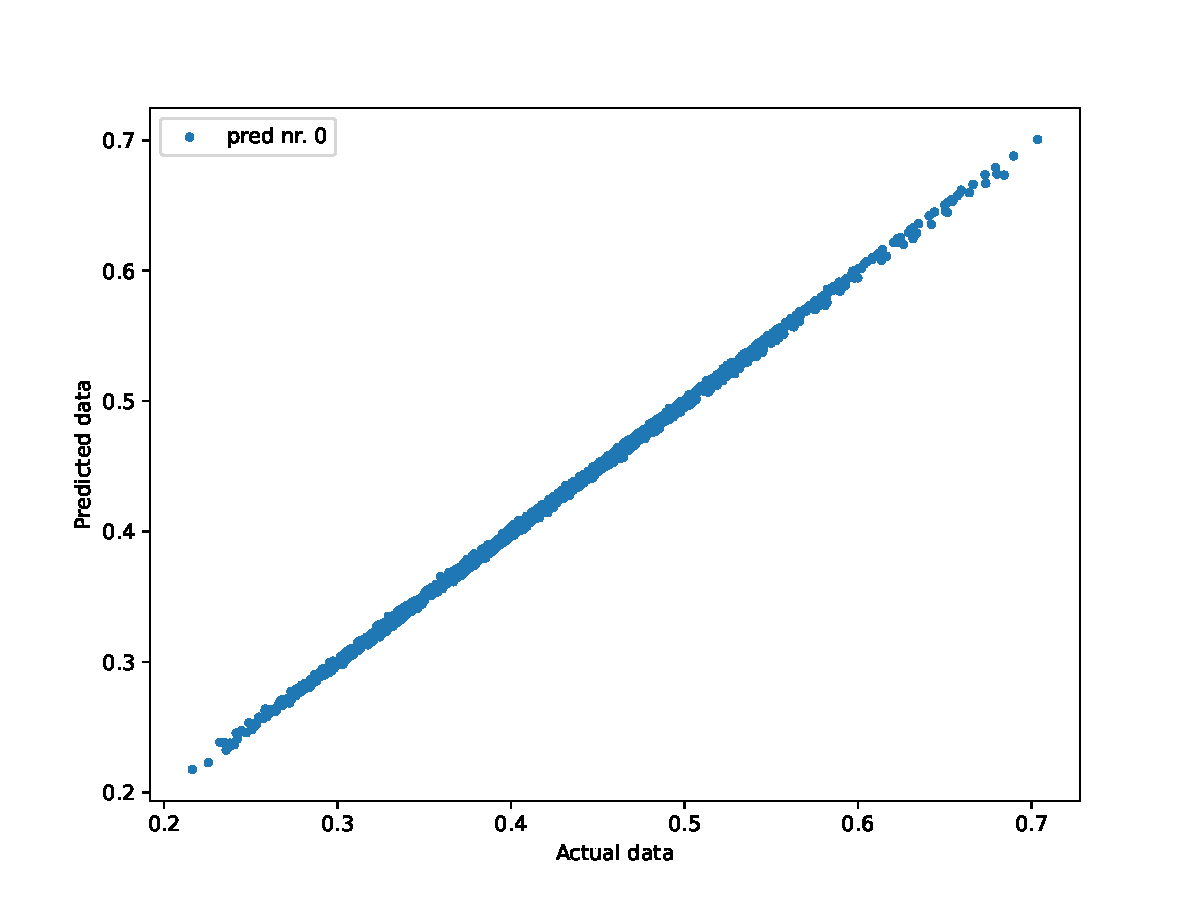
\includegraphics[width=0.8\textwidth]{figures/task2/final.pdf}
    \caption{Comparison between the predicted $CF$ values from the training set and the actual $CF$ values in the training set}
    \label{fig:task2}
\end{figure}

\section*{Task 3}
In this task the temperature data was fist normalized using min-max normalization. The temperature data was then structured so that consecutive temperature measurements are given for each starting time index. The training of the models was then done using the start of these sequences as input and the end as labels to approximate. A feed forward fully connected network was first used, but a network with an LSTM layer performed better on both series of temperatures. Ensemble training was then performed to select the optimal hyperparameters among input length, optimizer, learning rate, regularization and neurons. The final model was trained 5 times, and the lowest validation error was chosen. The predictions for each temperature series can be found in Figure \ref{fig:task3}
\begin{figure}[t]
  \begin{subfigure}[b]{0.5\textwidth}
    \centering
    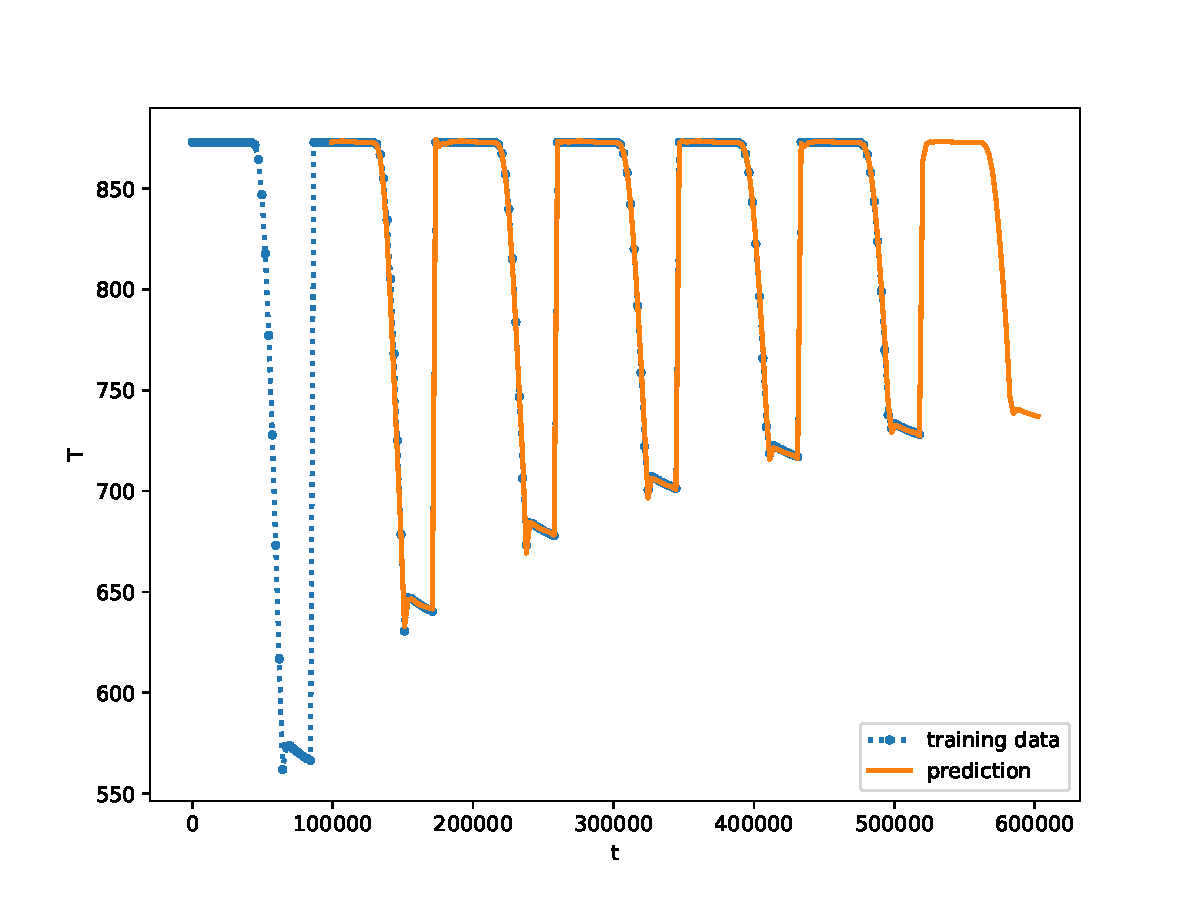
\includegraphics[width=\linewidth]{figures/task3/final_tf0.pdf}
    \caption{$T_f^0$}
    \label{fig:task3a}
  \end{subfigure}
  \begin{subfigure}[b]{0.5\textwidth}
    \centering
    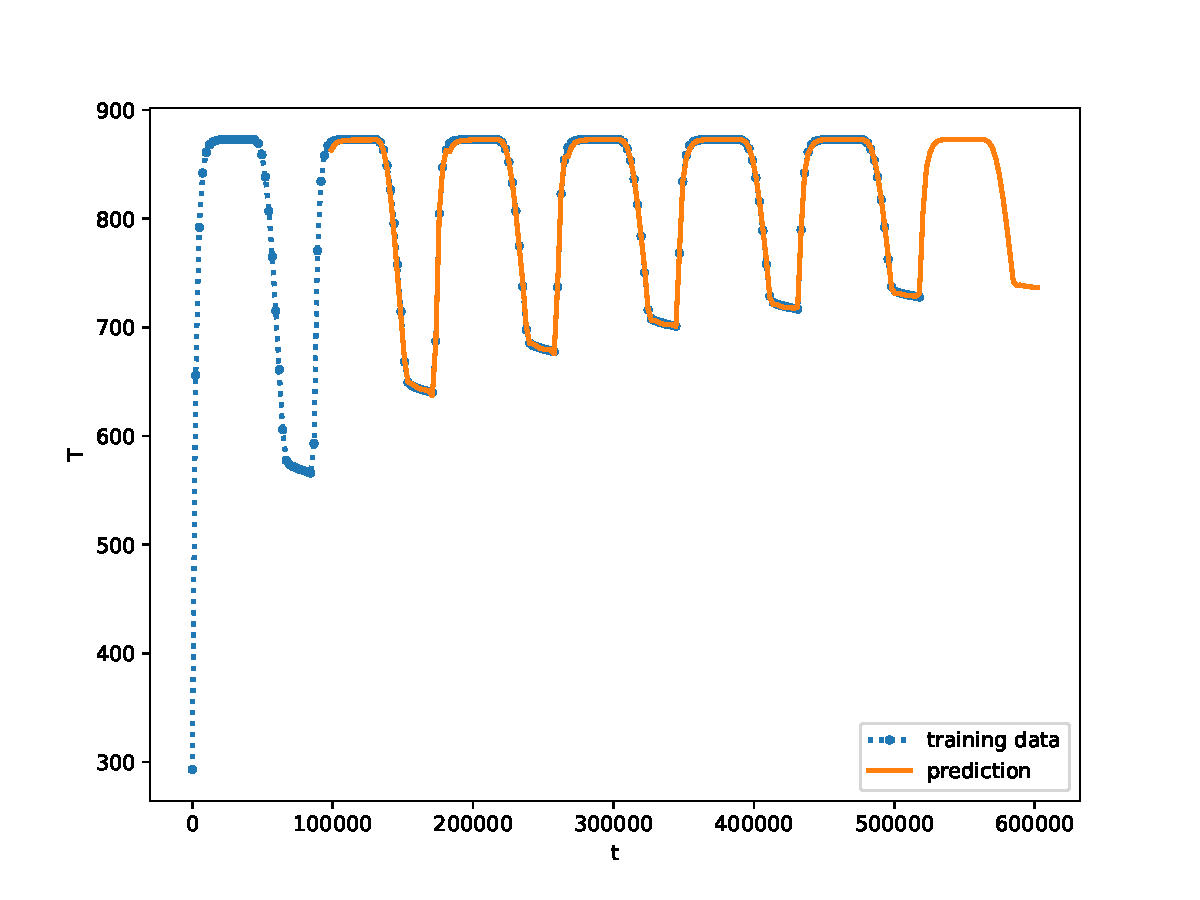
\includegraphics[width=\linewidth]{figures/task3/final_ts0.pdf}
    \caption{$T_s^0$}
    \label{fig:task3b}
  \end{subfigure}
  \caption{Training points and predictions by the model}
  \label{fig:task3}
\end{figure}

\section*{Task 4}
In this task the training data $S$ where first normalized to the domain $[0,1]^3$, using min-max scaling. Using the normalized data a feed forward neural network $T^L_{\theta}(t, u)$ was then trained to approximate the map $T^L(t, u)$. The model depends on several hyperparameters including layers, neurons, activation function, optimization algorithm, learning rate, and regularization. The chosen parameters were chosen with ensemble training using cross validation error as a selection criterion.

With a model selected, the noisy data $(T_{f,j}^{L,*}, t_j)_{j=1}^{N}$ was used to define the loss function
\begin{equation}
	G(u) = \sum_{j=0}^{N}{(T_{f,j}^{L,*} - T_{\theta}(t_j,u))^2}.
\end{equation}
The optimization problem was then solved by SGD with projected gradient. The resulting data are visualized in Figure \ref{fig:task4}
\begin{figure}[t]
    \centering
    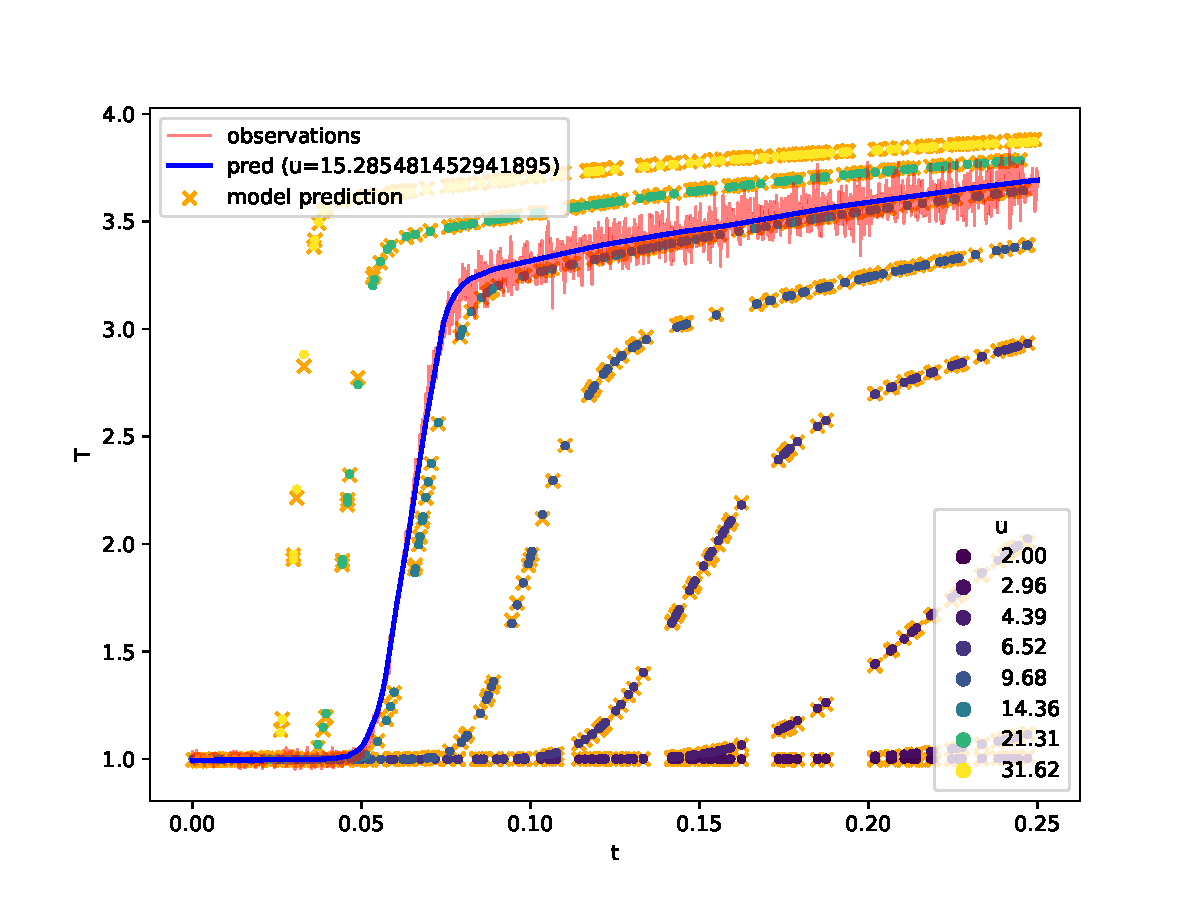
\includegraphics[width=0.8\textwidth]{figures/task4/final.pdf}
    \caption{The figure shows training values colored by $u$ and the predictions made by the chosen model. The noisy measurements are also depicted with a blue line noting the approximated curve $(T,t)$ for the given $u$}
    \label{fig:task4}
\end{figure}

\section*{Task 5}
In this task the control parameters $(v,D)$ in training set $S$ where first normalized to the domain $[0,1]^2$,  with maximum and minimum parameters given as $[2,20]\times[50,400]$. Using the normalized data a feed forward neural network $CF_{\theta}(D, v)$ was then trained to approximate the map $CF(D, v)$. The model depends on several hyperparameters including layers, neurons, activation function, optimization algorithm, learning rate, and regularization. The chosen parameters were chosen with ensemble training using cross validation error as a selection criterion.  The final model was trained 5 times, and the lowest validation error was chosen. 

Once a suitable model was selected the loss function
\begin{equation}
	G(D,v) = (CF_{ref}- CF_{\theta}(D,v))^2
\end{equation}
was minimized using SGD with projected gradient 1000 starting points as in the DNNopt\cite{Lye_2021} procedure. The starting points where chosen as the elements in a Sobol sequence in $\R^2$ . The optimization algorithm chosen was SGD with projected gradient. To speed up the optimization, loss was summed over all points, which enabled optimization of all the points simultaneously. The final model was trained 5 times, and the lowest validation error was chosen. The curve of optimal points can be viewed in Figure \ref{fig:task5}

\begin{figure}[t]
    \centering
    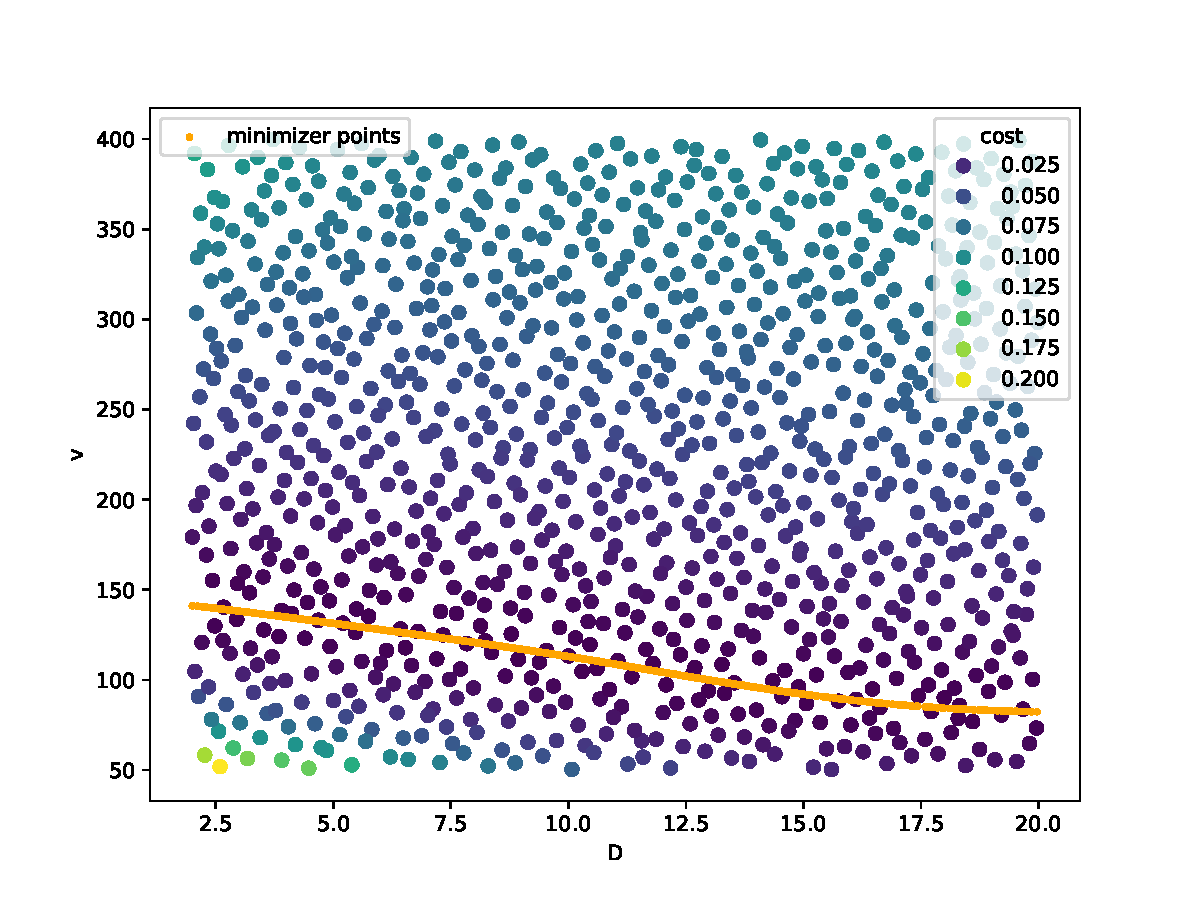
\includegraphics[width=0.8\textwidth]{figures/task5/final_optim_points.pdf}
    \caption{Optimal curve of $(D^*,v^*)$ values. The initial Sobol points are also shown with the corresponding $G$ value}
    \label{fig:task5}
\end{figure}

\section*{Appendix}
The code for this project can be found at \url{https://github.com/alexarntzen/deepthermal}

\FloatBarrier
\printbibliography
\end{document}


